\documentclass{beamer}

%% Fonts and encodings
\usepackage{multicol}
\usepackage{mathabx}
\usepackage[scaled]{helvet}
\usepackage{color}
\usepackage{lmodern}
\usepackage{eulervm}
\usepackage{wasysym}
\usefonttheme[onlymath]{serif}
\usefonttheme{professionalfonts}
\usefonttheme{structurebold}
\hypersetup{backref}
\usepackage{bm}
%\usepackage[utf8x]{inputenc}
\usepackage{natbib}
\setlength{\bibsep}{0.0pt}
\usepackage{booktabs}
%% Color & Theme
\definecolor{SUblue}{RGB}{0,0,180}
\usecolortheme[RGB={0,0,180}]{structure}
\usetheme{Boadilla}
\setbeamertemplate{navigation symbols}{}
\setbeamerfont{title}{size=\large}
\setbeamerfont{frametitle}{size=\normalsize}
\setbeamerfont{framesubtitle}{size=\small, shape =$\color{violet}{\looparrowdownright}~$}
\setbeamercolor{title}{fg=white, bg= SUblue!75!green}
\setbeamercolor{framesubtitle}{fg=violet}

%% Reduce the left margin
% \setlength{\leftmargini}{5pt}
% \setbeamertemplate{frametitle}
% {
% \raggedright\insertframetitle%
% }


\title[Bayesian Multivariate Density Estimation]{{Bayesian
   Multivariate Density Estimation}}
\subtitle{\small{--- with the approach of copula methods}}

\author[Feng Li]{\textbf{Feng Li}}
\institute[Stockholm University]{\textbf{Department of
    Statistics, Stockholm University}}
\date{\color{SUblue}{ \textbf{April, 2013}}}

\begin{document}

%% Title page
\maketitle

%% Outline
\section*{Outline of the talk}
\begin{frame}
  \frametitle{Outline of the talk}
  \addtocounter{framenumber}{-1}
  \tableofcontents
\end{frame}

\section{Flexible density estimation}
\begin{frame}
  \frametitle{Flexible density estimation}
  \framesubtitle{Introduction}
  \begin{itemize}
  \item Density estimation consecrates on modeling the relationship between
the response $\bm{y}$ with covariates $\bm{x}$ with flexible density function
$f(\cdot)$
\begin{equation*}
  \label{eq:1}
  \bm{y} = f(\bm{x},{\theta})
\end{equation*}

\emph{flexible}: the density feature $\bm{\theta}$ are modeled in a flexible way.

\item An example: GLM: density estimation with flexible mean function $\eta(\mu) =
    \bm{X\beta} $ via the linkage.

\item Two main factors that influence the efficiency of the density estimation,
\begin{enumerate}
\item [(1)] choice of flexible densities, and
\item [(2)] ways of constructing densities features.
\end{enumerate}
\end{itemize}
\end{frame}

\section{The challenge in multivariate density estimation}
\begin{frame}
  \frametitle{Flexible density estimation}
  \framesubtitle{Univariate or multivariate}
\begin{itemize}
\item (Relevantly) simpler in univariate response
  \begin{itemize}
  \item  Mixture of experts
  \item  Nonparametric methods: kernel regression, splines...
  \end{itemize}

\item More tricky in the multivariate case

  \begin{itemize}
  \item Flexible multivariate density is difficult to construct \emph{per se}
  \item Not only modeling the density features in each marginal model
  \item But also multivariate correlations and other dependences need to take into account.
  \end{itemize}
\end{itemize}
\end{frame}

\begin{frame}
  \frametitle{Features of interest in multivariate densities}

Besides the features of interest in each marginal density, dependence is the
never ending story in multivariate densities.

  \begin{itemize}
  \item The general measure of correlation: \textbf{Kendall's $\tau$}
    \begin{equation*}
      \begin{split}
        \tau = & 4 \int \int F(x_1, x_2)dF(x_1,x_2)-1% = 4 \int \int C(u_1, u_2)dC(u_1,u_2)-1. \\
      \end{split}
    \end{equation*}

  \item The dependence in the tail
    \begin{equation*}
      \begin{split}
        \lambda_L = & \lim \limits_{u \to 0^{+}} Pr(X_1< F_1^{-1}(u)| X_2<F_2^{-1}(u))\\%= \lim \limits_{u \to 0^{+}} \frac{C(u,u)}{u}\\,
        \lambda_U=&\lim \limits_{u \to 1^{-}} Pr(X_1> F_1^{-1}(u)|
        X_2>F_2^{-1}(u))%= \lim \limits_{u \to 1^{-}} \frac{1-C(u,u)}{1-u}.\\
      \end{split}
    \end{equation*}
  \end{itemize}
However estimating these features are very difficult in standard multivariate
density settings. No general approach until the next slide.

\end{frame}

\begin{frame}
  \frametitle{Copulas}
  \begin{itemize}
  \item \textbf{Sklar's theorem}
    Let $H$ be a multi-dimensional distribution function with marginal
    distribution functions $F_1(x_1),...,F_m(x_m)$. Then there exists a
    function $C$ (\textbf{copula function}) such that
    \begin{equation*}
      \begin{split}
        H(x_1,...,x_m)= & C(F_1(x_1),...,F_m(x_m))\\
        =&C\left(\int_{-\infty}^{x_1}f(z_1)dz_1,...,\int_{-\infty}^{x_m}f(z_m)dz_m\right)=C(u_1,...,u_m).
      \end{split}
    \end{equation*}
\item Here is the magic
  \begin{equation*}
    \label{eq:2}
      \begin{split}
        \tau = & 4 \int \int F(x_1, x_2)dF(x_1,x_2)-1 = 4 \int \int C(u_1, u_2)dC(u_1,u_2)-1. \\
        \lambda_L = & \lim \limits_{u \to 0^{+}} Pr(X_1< F_1^{-1}(u)| X_2<F_2^{-1}(u))= \lim \limits_{u \to 0^{+}} \frac{C(u,u)}{u}\\,
        \lambda_U=&\lim \limits_{u \to 1^{-}} Pr(X_1> F_1^{-1}(u)|
        X_2>F_2^{-1}(u))= \lim \limits_{u \to 1^{-}} \frac{1-C(u,u)}{1-u}.\\
      \end{split}
  \end{equation*}

  \end{itemize}
\end{frame}

\section{The multivariate density estimation with copulas}
\begin{frame}
  \frametitle{The covariate-dependent copula model}
  \begin{itemize}
  \item The multivariate density (in terms of copulas) features to be connected with observed data information. In particular, correlation and tail-dependence are the two concepts of interest in various of situation,
\begin{equation*}
  \begin{split}
 \tau=\eta_{\tau}^{-1}(\bm{X}\bm{\beta}_{\tau}),\text{ and } \lambda=\eta_{\lambda}^{-1}(\bm{X}\bm{\beta}_{\lambda})
  \end{split}
\end{equation*}

\item The marginal models are constructed via the usual approach in univariate
  density (mixtures, splines, etc)

\item The Bayesian approach
  \begin{equation*}
    \begin{split}\log p(\{\bm{\beta},\bm{\mathcal{I}}\}|\bm{Y},\bm{X})= & \mathrm{constant}+\sum\nolimits _{j=1}^{M}\log p(\bm{Y}_{.j}|\{\bm{\beta},\bm{\mathcal{I}}\}_{j},\bm{X}_{j})\\
 & +\log\mathcal{L}_{C}(\bm{u}|\{\bm{\beta},\bm{\mathcal{I}}\}_{C},\bm{Y},\bm{X})+\log p(\{\bm{\beta},\bm{\mathcal{I}}\})
\end{split}
  \end{equation*}
  \begin{itemize}
  \item Efficient MCMC to sample the posterior (tailored Metropolis-Hastings)
  \item Bayesian variable selection is integrate seamlessly.
  \item Model comparison and copula density selection via predictive
    likelihood.
  \end{itemize}
\end{itemize}
\end{frame}

% \section{Application with financial data}
% \begin{frame}
% \frametitle{The data in the application}

% The S\&P100 index includes the largest
% and most established companies which is a subset of the well-known SP500 index
% in stock market. The S\&P600 index covers the small capitalization companies
% which present the possibility of greater capital appreciation, but at greater
% risk.
% \begin{table}
%   % \caption{Description of variables in the S\&P100 and S\&P600 data.}
%   % \label{tab:sp-covariates}
%   \centering
% \resizebox{0.8\textwidth}{!}{
%     \begin{tabular}{l p{0.8\textwidth}l}
%       \toprule
% %      Variable& Description\\
% %      \midrule
%       \textsf{Return} & Daily return $y_t=100\log(p_t/p_{t-1})$ where $p_t$ is the
%       closing price.\\
%       \\
%       \textsf{RM1}& Return of last day.\\
%       \textsf{RM5}& Return of last week.\\
%       \textsf{RM20}& Return of last month.\\
%       \textsf{CloseAbs95}&Geometrically decaying average of absolute returns
%       $(1-\rho)\sum \nolimits_{s=0}^{\infty} \rho^s|y_{t-2-s}|$ with $\rho=0.95$.\\
%       \textsf{CloseAbs80}&Geometrically decaying average of past absolute returns with $\rho=0.80$.\\
%       \textsf{MaxMin95}&Measure of volatility $(1-\rho)\sum
%       \nolimits_{s=0}^{\infty} \rho^s(\log(p_{t-1-s}^h)-\log(p_{t-1-s}^l))$ with $\rho=0.95$,
%       where $p^h$ and $p^l$ are the highest and lowest prices.\\
%       \textsf{MaxMin80}&Measure of volatility with $\rho=0.80$.\\
%       \textsf{CloseSqr95}& Geometrically decaying average of returns  $((1-\rho)\sum \nolimits_{s=0}^{\infty}
%       \rho^sy_{t-2-s}^2)^{1/2}$ with $\rho=0.95$.\\
%       \textsf{CloseSqr80}& Geometrically decaying average of returns with $\rho=0.80$.\\
%       \bottomrule
%     \end{tabular}
% }
% \end{table}


% \end{frame}

% \begin{frame}
%   \frametitle{The model in the application}
%   \begin{itemize}

%   \item In the marginal models we us asymmetric student-t densities, we allow
%     the location parameter $\mu$, scale parameter $\phi$ skewness parameter
%     $\kappa$ and degrees of freedom $\nu$ are connected to covariates as
%     \begin{itemize}
%     \item $\mu_{ij}= x_{ij}'\beta_{\mu_j}$
%     \item $ \phi_{ij}= \exp( x_{ij}'\beta_{\phi_j})$
%     \item $\nu_{ij}=\exp( x_{ij}'\beta_{\nu_j})$
%     \item $\kappa_{ij} =\exp( x_{ij}'\beta_{\lambda_j})$,
%       for $i = 1,...,n$, $j = 1,...,M$
%     \end{itemize}
% \item The copula density is called the Joe-Clayton copula. All covariates in
%   the marginal model are included in the copula features Kendall's $\tau$ and
%   tail-dependence parameter $\lambda$.
%   \end{itemize}
% \end{frame}

% \begin{frame}[plain]
%   \begin{figure}
%     \centering
%     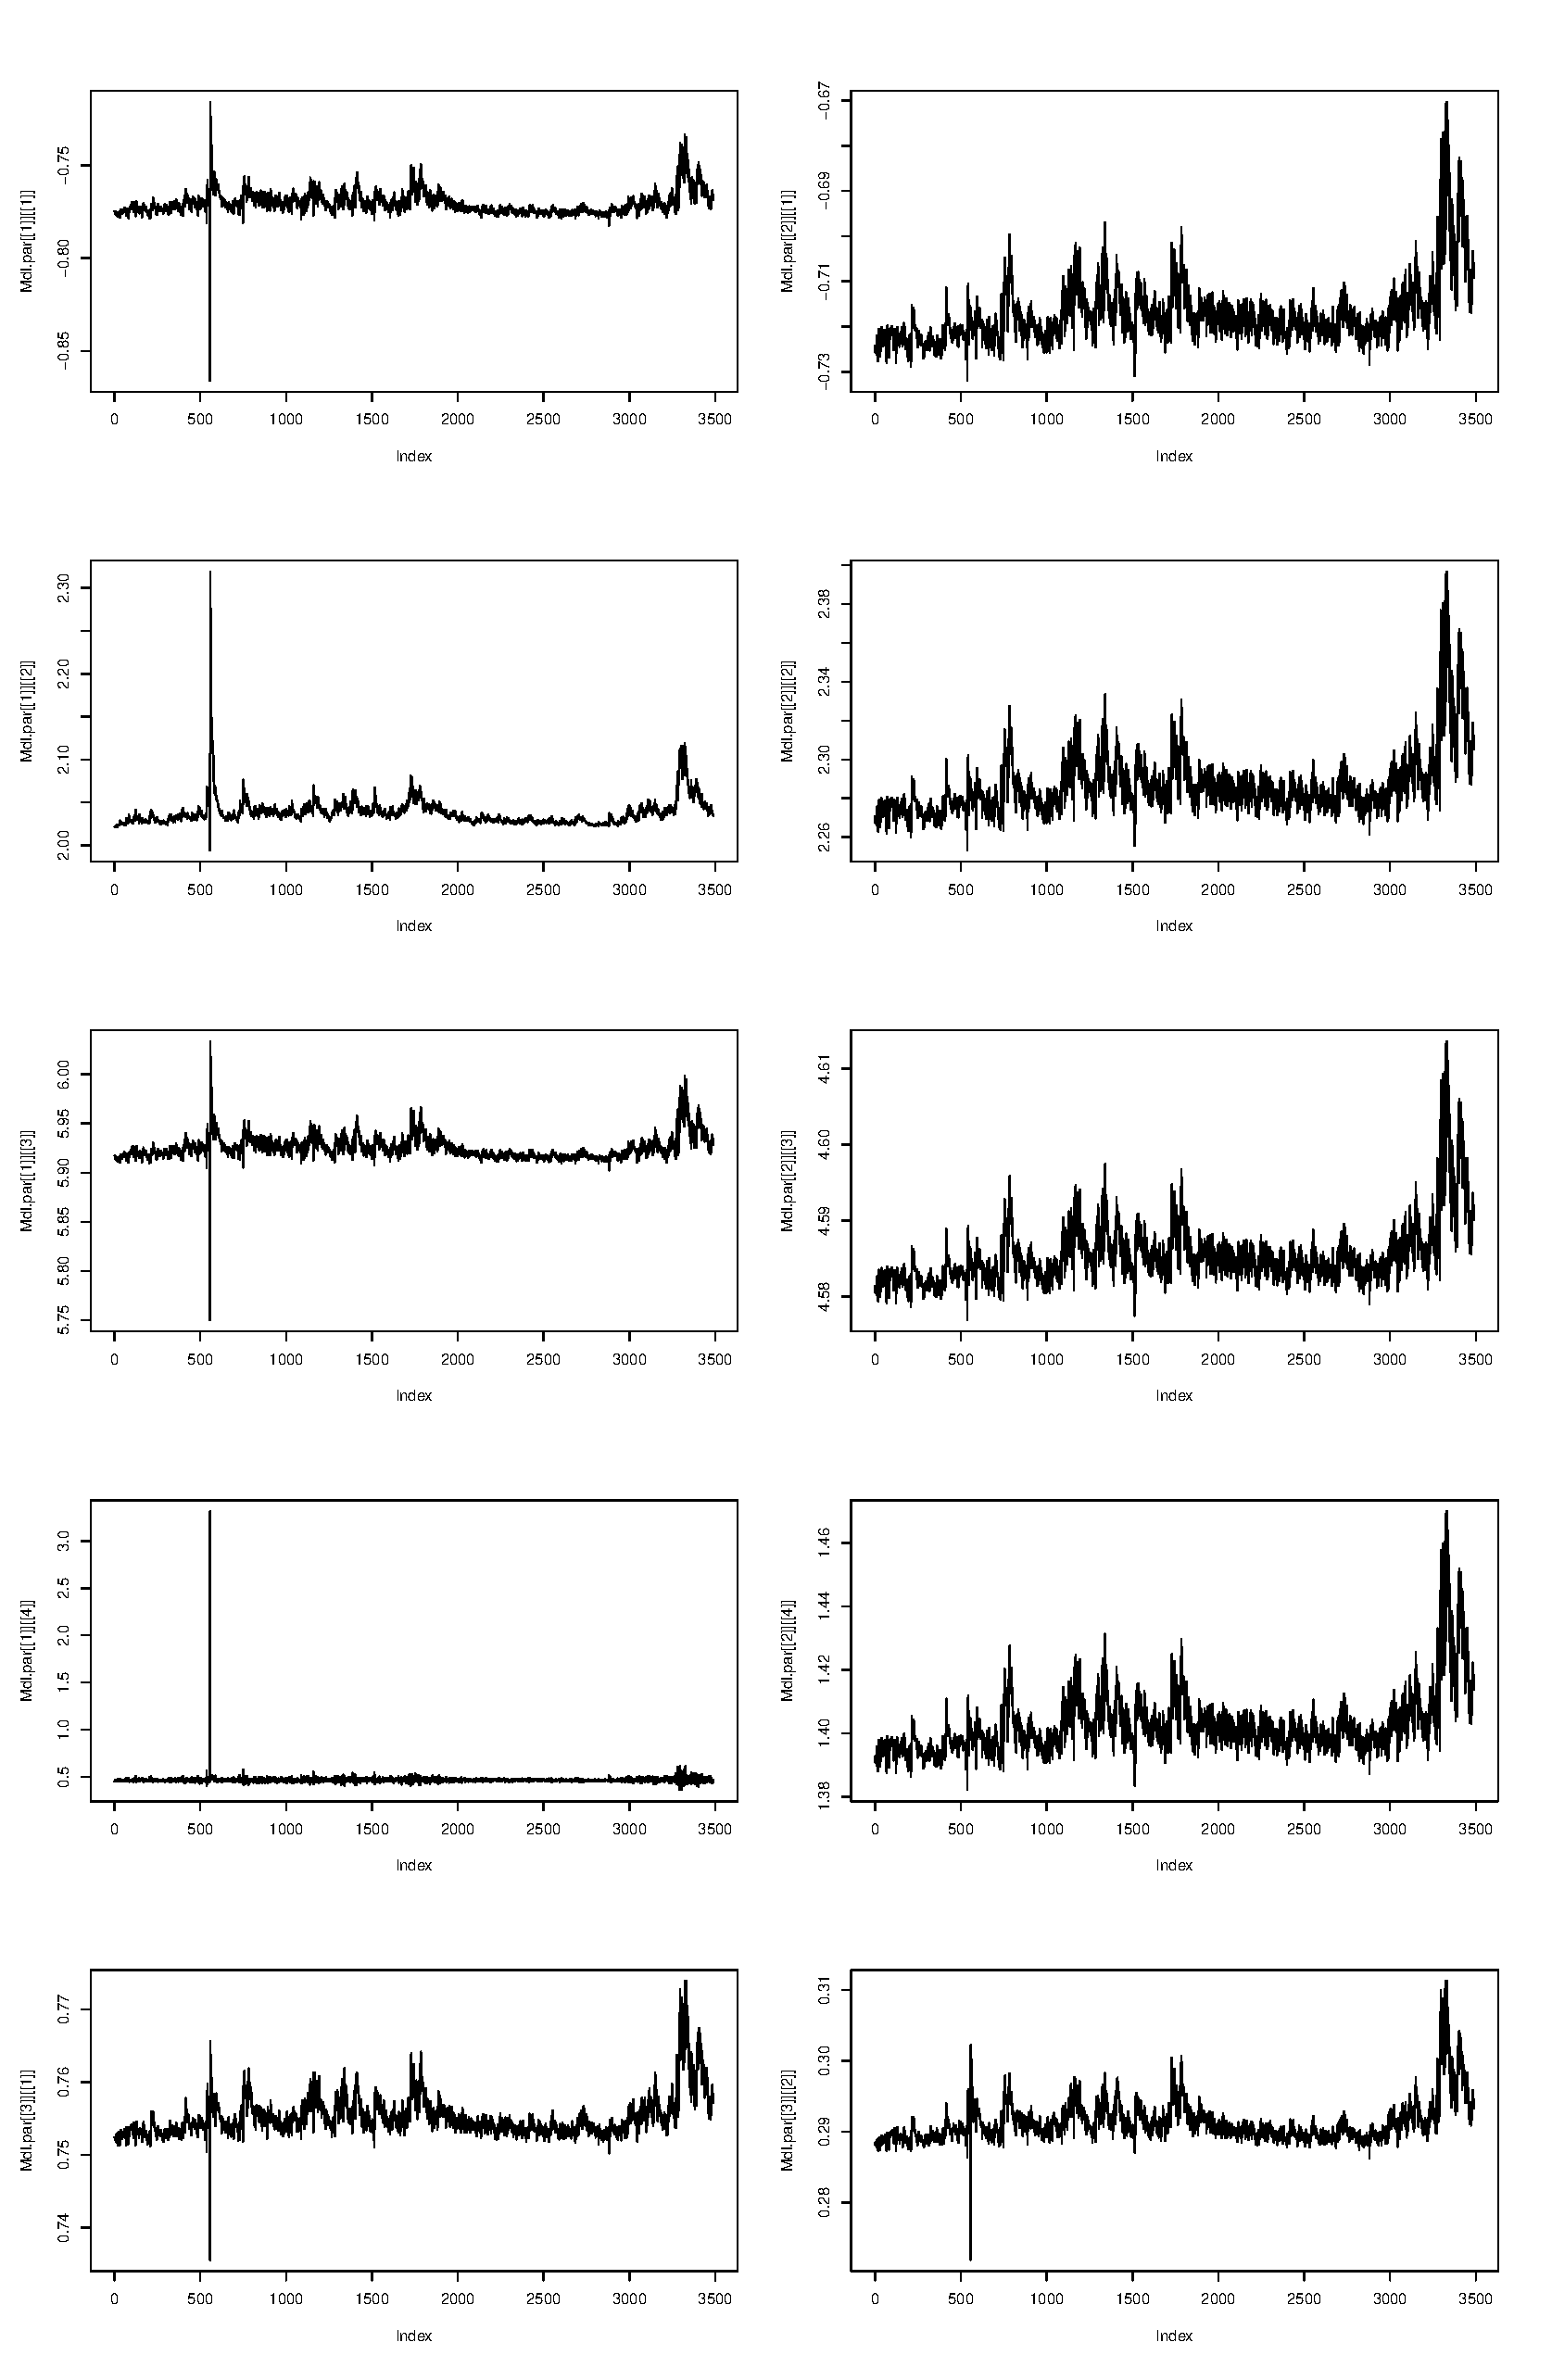
\includegraphics[height=1.05\textheight]{SP100-SP600-post}
%   \end{figure}

% \end{frame}

\begin{frame}[plain]
  \addtocounter{framenumber}{-1}
  \begin{center}
    {\color{SUblue} \textbf{\Huge Thank you!}}

\vspace{1cm}

{\texttt{\textbf{feng.li@stat.su.se}}}
  \end{center}
\end{frame}

\end{document}
